% Overleaf無料枠でのタイムアウト回避のため、upLaTeX + dvipdfmx を使用する
% 章を必ず右ページ(奇数)から開始する挙動により空白ページが挿入されるのを避ける
\documentclass[a4paper,12pt,openany]{jsreport}

% jsreport環境によっては章開始時に \cleardoublepage が使われ、白紙ページが挿入されることがある。
% これを確実に防ぐため、\cleardoublepage を \clearpage と同等にする。
\let\cleardoublepage\clearpage

% ---- Page / typography ----
\usepackage[margin=25mm]{geometry}
\usepackage{setspace}
\onehalfspacing

% ---- Math / figures ----
\usepackage{amsmath,amssymb}
\usepackage[dvipdfmx]{graphicx}
% numeric citation formatting (e.g., [1], [2,3])
\usepackage{cite}
% NOTE: caption系はクラスによって警告が出ることがあるため、必要になったら追加する
% \usepackage{caption}
% \usepackage{subcaption}

% ---- Links ----
\usepackage[dvipdfmx,hidelinks]{hyperref}
\usepackage{pxjahyper}
\usepackage{bookmark}
% PDF提出用：リンクを黒（色・枠線なし）で出力する
% ※リンク自体（クリック可能）は維持される
\hypersetup{hidelinks}

% ---- References ----
% Overleaf無料枠でのタイムアウト回避のため、まずはbiber不要のthebibliographyを使用する。
% 文献が増えてbib管理を自動化したくなった段階で、biblatex/biberに切り替える。

% ---- TOC depth (edit if needed) ----
% 0: chapter, 1: section (1.1), 2: subsection (2.1.1), 3: subsubsection (2.1.1.1)
\setcounter{tocdepth}{1}

\begin{document}

% ---- Cover (大学フォーマットに合わせて編集) ----
\thispagestyle{empty}
\begin{center}
{\LARGE 卒業研究論文\par}
\vspace{6mm}
{\large （2025年度）\par}
\vspace{18mm}

{\Large 題目\par}
\vspace{4mm}
日本株市場におけるニュースの新規性（Novelty）と株価リスクの関係\par
\vspace{2mm}
\rule{0.9\textwidth}{0.4pt}\par
\vspace{10mm}

\begin{tabular}{p{0.25\textwidth}p{0.65\textwidth}}
指導教員 & 野口 怜 \\[2mm]
学籍番号 & 8722014 \\[2mm]
氏名 & 石川 純 \\
\end{tabular}

\vfill
{\large 東京理科大学 経営学部\par}
\end{center}
\clearpage

% ---- TOC ----
\pagenumbering{roman}
\tableofcontents
\clearpage
\pagenumbering{arabic}

% ---- Chapters ----
\chapter[序論（諸言：背景と目的）]{諸言}

\section{背景}

企業が投資家に提供する情報は、決算短信や適時開示、報道記事など多様であるが、その中でも有価証券報告書は、企業の経営実態や将来見通しに関する相対的に体系立った情報を網羅的に含む点で重要である。とりわけ「事業等のリスク」欄は、企業が認識する主要なリスク要因を言語で整理し、継続的に開示するセクションであり、投資家が企業の不確実性を評価する上で中心的な手がかりになり得る。一方で実務的には、当該セクションが前年と類似した表現の反復になりやすいこと（いわゆるコピペ）も指摘されており、開示の“量”だけではなく、“内容がどれだけ更新されているか”という質的側面を捉える必要性が高まっている。開示文が更新される局面、すなわち前年には見られなかったリスク要因の追加や、強調点の変化、具体化・詳細化が生じる局面では、投資家が受け取る情報の新規性が高い可能性がある。一般に投資家の注意には制約があるため、反復的な記述よりも、新規性を伴う記述の方が市場参加者の注目を集め、売買行動を誘発しやすいと考えられる。また、新たなリスク情報は将来のキャッシュフローや分散に関する不確実性の認識を変化させ得るため、短期的には株価の不確実性（予想外の価格変動）の増大として観察される可能性がある。他方で、新規な開示が不確実性を単に高めるとは限らず、リスクの所在を明確化することで投資家の理解が進み、反応が限定的となる可能性もある。したがって、リスク開示の新規性が市場の反応に与える影響は理論的に一意ではなく、実証的に検証すべき論点である。先行研究では、開示文の分量や語調、可読性、あるいは定型性（ボイラープレート性）に着目した分析が蓄積されてきた。しかし、日本企業の有価証券報告書を対象に、「事業等のリスク」欄の年度間の内容変化そのものを定量化し、その変化が開示日周辺の市場反応（例：投資家の注目度や不確実性）とどのように関係するかを検証した研究は依然として限定的である。本研究は、リスク記述をチャンク単位に分割し、前年記述との意味的類似度にもとづいて開示の新規性（変化度）を定量化した上で、提出日をイベント日とするイベントスタディ枠組みにより、短期の市場反応を検証する。これにより、リスク開示が「形式的に存在する情報」なのか、それとも「更新（新規性）を通じて市場参加者の行動や不確実性に影響する情報」なのかを明らかにすることを目的とする。

\section{関連研究}

本研究は、有価証券報告書におけるリスク開示研究と、開示テキストの更新（新規性）を捉えるテキスト分析、さらに提出日を基準としたイベントスタディによる市場反応分析を接続するものである。
以下では、（1）リスク開示の情報内容、（2）リスク開示“更新”の検出、（3）日本語有報研究、（4）LLM/埋め込みを用いたテキスト指標化、の観点から先行研究を整理し、本研究の位置づけを示す。なお、会計・ファイナンス領域におけるテキスト分析の体系的整理としては \cite{LoughranMcDonald2016} がある。

まず、リスク開示が企業の実態や市場のリスク認識と関連し得ることは、リスク語辞書や頻度分析を通じて示されてきた。初期研究として、訴訟リスクと任意開示の関係に着目し、開示文書における注意喚起的な表現（cautionary language）の役割を検討する枠組みが提示されている\cite{NelsonPritchard2007}。
その後、米国 10-K を対象に、リスク関連語の頻度やリスク開示の量的指標が、株式リスク（β やボラティリティ）や提出直後の市場反応（CAR）と結びつくことが報告され、リスク開示が市場参加者にとって情報価値を持つ可能性が示されている\cite{Campbell2014}。

一方で、リスク開示は「リスクを増やした」という悪材料の通知であるだけでなく、情報環境の改善として評価され得るため、開示内容の質（とりわけ具体性）に着目した研究も重要である。具体性の高いリスク開示ほど提出時 CAR が正となり、またアナリスト予想精度の改善と関連することが示されており、開示の“質”が市場反応を左右し得る点が示唆される\cite{HopeHuLu2016}。

次に、本研究が中心的に扱う「新規性（更新）」に関して、単なる分量や頻度ではなく、“前年から何が変わったか”を捉える必要性が指摘されてきた。四半期報告（10-Q）のリスク要因更新をテキストマッチングで検出し、更新企業で提出直後に株価下落が観察されること、ただし反応が一部遅れて生じ得ることを示す研究は、リスク開示の更新が市場に新情報を与えるという解釈と整合的である\cite{Filzen2015}。
また、リスク要因の追加・削除といった“変化”が不確実性指標（例：VRP 等）と結びつくことを示す研究は、リスク開示の変化そのものが投資家の将来リスク認識に影響し得ることを示唆する\cite{Lyle2023}。さらに、開示テキストの内容が投資家のリスク認識と結びつくことも報告されている\cite{KravetMuslu2013}。
加えて、開示テキストの構造的変化や論点の推移を、トピックモデル（例：Latent Dirichlet Allocation）により捉える研究も存在し、開示内容の「変化」を定量的に扱うという点で本研究の問題意識と接続する\cite{Dyer2017}。

日本の有価証券報告書「事業等のリスク」欄に関しても、テキスト分析に基づく蓄積が存在する。たとえば開示量（語数等）と情報の非対称性の低下（アナリスト予想精度の向上）との関連が示される一方、量の増大が内容の平板化を伴い得る点、前年比較や具体的記載の必要性が示唆されている\cite{Noda2016}。
さらに、日本語のリスク辞書（専門家辞書＋機械学習辞書）を用いた研究では、リスク関連語の出現確率が株価リスク指標（ボラティリティ）と正に相関することが示される一方、前年比の変化のみではリスク変動を十分説明できないことが報告されている\cite{SatoIkedaInoue2021}。この結果は、「頻度の前年差分」だけではリスク構造の変化を捉えきれない可能性、すなわち“意味的な更新”を捉える指標の必要性を示唆する。

以上を踏まえると、先行研究は（i）リスク開示が市場・リスク指標と関連し得ること、（ii）開示の質（具体性等）が市場反応を左右し得ること、（iii）開示の更新（追加・削除）が不確実性と結びつき得ることを示してきた。しかし、日本企業の有報「事業等のリスク」欄について、年度間の意味的更新を安定的に定量化し、提出日をイベント日として市場反応を多面的に検証する枠組みは依然として限定的である。
そこで本研究は、リスク記述をチャンク単位に分割し、前年チャンク群との最大類似度に基づく変化度（新規性）指標を構築したうえで、提出日前後の短期反応をイベントスタディで捉える。特に、価格反応（CAR）に加えて、投資家の注目度を表す出来高指標や、不確実性を表す異常収益の絶対値集計等を併用することで、リスク開示の新規性が「注目」「不確実性」「価格」のどこに強く現れるかを識別する点に本研究の特徴がある。

\section{研究目的・研究課題と仮説}

\subsection{研究目的}

本研究の目的は、有価証券報告書「事業等のリスク」欄における記述の新規性（前年からの内容更新）をテキスト類似度に基づいて定量化し、その新規性が提出日周辺の資本市場反応に与える影響を実証的に明らかにすることである。とくに、リスク開示の影響は価格反応（CAR）だけに表れるとは限らないため、本研究では、価格反応に加えて投資家の注目度（出来高）および不確実性の高まり（異常収益の絶対値集計等）を併用し、リスク開示の新規性が市場のどの側面に強く反映されるかを検証する。

\subsection{研究課題（Research Question）}

上記目的を踏まえ、本研究は以下の研究課題を設定する。

\begin{itemize}
  \item RQ1：有報「事業等のリスク」欄の新規性が高いほど、提出日周辺で投資家の注目度（出来高）は高まるか。
  \item RQ2：新規性が高いほど、提出日周辺で市場の不確実性（予想外の価格変動の大きさ）は高まるか。
  \item RQ3：新規性が高いほど、提出日周辺で株価はネガティブに反応するか（CAR は低下するか）。
\end{itemize}

\subsection{仮説}

リスク開示の更新は投資家にとって新情報であり、注意の配分や解釈のばらつきを通じて取引活発化や不確実性の上昇をもたらし得る。また、リスク要因の追加・強調は一般にネガティブ情報として受け止められやすい。したがって、本研究では以下の仮説を設定する。

\begin{itemize}
  \item H1（注目度）：リスク開示の新規性が高いほど、提出日周辺の異常出来高（注目度）は増加する。
  \item H2（不確実性）：リスク開示の新規性が高いほど、提出日周辺の不確実性指標（例：異常収益の絶対値集計）は増加する。
  \item H3（価格反応）：リスク開示の新規性が高いほど、提出日周辺のCAR は低下する。
\end{itemize}

\subsection{検証の概要}

本研究では、リスク記述をチャンク単位に分割し、前年のチャンク集合との最大類似度から変化度（新規性）を算出することで説明変数を構成する。アウトカムは、（i）市場調整した異常出来高（注目度）、（ii）市場モデルに基づく異常収益の絶対値集計（不確実性）、（iii）市場モデル CAR（価格反応）とし、提出日をイベント日とするイベントスタディおよび回帰分析により、上記仮説を検証する。

\section{本研究の新規性・貢献}

本研究の新規性・貢献は以下のとおりである。第一に、有価証券報告書「事業等のリスク」欄における開示内容について、単なる文量やリスク語頻度ではなく、前年からの内容更新（新規性）に焦点を当てる点に新規性がある。リスク開示は年次で反復されやすく、記述の定型性が高い場合には、開示“量”が増えても情報価値が増えない可能性がある。そのため、開示が実際にどの程度更新されているのかを定量化し、市場がその更新に反応するかを検証することは、リスク開示の有用性を評価する上で重要である。第二に、本研究は新規性の測定において、リスク記述をチャンク単位に分割し、前年記述との意味的類似度に基づく変化度指標を構築する。これにより、表現の揺れや言い換えが存在しても、内容としての近さ・遠さを一定程度考慮した形で「更新」を捉えることができ、従来の単純な頻度差分では捉えにくい意味的変化を扱える点に方法論的貢献がある。第三に、市場反応を価格反応（CAR）だけに限定せず、投資家の注目度（出来高）および不確実性（異常収益の絶対値集計等）を併用して多面的に検証する。リスク開示の更新は、直ちに価格に強く反映されるとは限らず、まず注意の喚起や解釈のばらつきとして現れる可能性がある。本研究の設計は、リスク開示新規性が市場のどの側面に表れやすいかを識別し、実証結果の解釈可能性を高める。以上により、本研究は、日本企業の有報「事業等のリスク」欄を対象に、開示の“更新（新規性）”という質的側面が市場参加者の反応とどのように結びつくかを明らかにし、開示実務および投資家の情報処理に関する理解に資する知見を提供する。

\section{論文の構成}

本論文の構成は次のとおりである。第 1 章では研究背景、先行研究、研究目的・仮説、ならびに本研究の貢献を示した。第 2 章ではデータ、変数定義、新規性指標の構築方法、およびイベントスタディと回帰分析の設計を説明する。第 3章では実証結果を提示し、第 4 章で結果の解釈、含意、限界点を考察する。最後に第 5 章で結論と今後の課題を述べる。

\chapter[研究方法（データと分析設計）]{研究方法}

本章では、本研究で用いるデータ、変数定義、新規性（Novelty）指標の構築方法、ならびに提出日をイベント日とするイベントスタディと回帰分析の設計を説明する。具体的には、まず有価証券報告書から「事業等のリスク」欄を抽出し、年度間比較が可能な形に整形する。次に、リスク記述をチャンク単位に分割し、前年記述との意味的類似度に基づいて内容更新の度合い（新規性）を定量化する。最後に、提出日周辺における市場反応を、価格反応

（CAR）に加えて注目度（出来高）および不確実性指標で多面的に測定し、新規性指標との関連を検証する。

\section{データ}

\subsection{企業・期間}

本研究は、日本の上場企業を対象とし、一定期間に提出された有価証券報告書を分析対象とする。サンプルは、提出企業のうち株価データおよび統制変数が取得可能であり、かつ前年の有価証券報告書が存在して年度間比較が可能な企業・年度に限定する。

\subsection{文書データ（有価証券報告書）}

文書データとして、有価証券報告書から「事業等のリスク」欄の本文を取得する。取得は電子開示システム（EDINET）により提供される提出書類データを用い、機械的に当該セクションを抽出したうえで、分析可能なテキストへ変換する。抽出の段階では、年度間比較の妨げとなる不要な装飾情報（例：HTML 由来のタグ、記号の過剰な連続、機械抽出のノイズ）を除去し、同一企業について前年との対応づけが可能な形で整形する。

\subsection{市場データ（株価・出来高）}

市場データとして、イベントスタディに必要な日次株価・出来高データを取得する。株価データは、提出日をイベント日としてイベント窓における異常収益を算出するために用いる。また、投資家の注目度を捉えるため、出来高を市場水準で調整した異常出来高指標を構築する。さらに、企業特性による交絡を抑えるため、規模や収益性、財務レバレッジ等の統制変数を取得し、回帰分析に組み込む。

\section{変数定義}

\subsection{説明変数：リスク開示の新規性（Novelty）}

本研究の中心的な説明変数は、有価証券報告書「事業等のリスク」欄における記述の新規性（前年からの内容更新の度合い）である。新規性は、当該セクションのテキストを一定単位（チャンク）に分割したうえで、前年テキストとの意味的類似度にもとづいて定量化する（構築方法の詳細は 2.3 で述べる）。本研究では、全体の新規性を表す指標（例：change\_topk）を基本とし、必要に応じてカテゴリ別の新規性指標も用いる。

\subsection{被説明変数（アウトカム）}

提出日をイベント日とし、イベント窓における市場反応を以下の 3 指標で測定する。

\begin{itemize}

  \item 注目度（出来高）：abvol\_mkt

\end{itemize}

市場平均出来高で調整した出来高（対数変換した出来高等）をイベント窓で集計した指標であり、情報に対する投資家の注意（attention）の高まりを捉える代理変数と位置づける。

\begin{itemize}

  \item 不確実性：vol\_abs

\end{itemize}

市場モデルに基づく異常収益（AR）の絶対値をイベント窓で合計した指標（\(\sum \lvert AR \rvert\)）であり、開示を受けた短期の不確実性・解釈のばらつきの大きさを捉える代理変数と位置づける。

\begin{itemize}

  \item 価格反応（参考）：car\_mm

\end{itemize}

市場モデルに基づく累積異常収益率（CAR）であり、開示が株価水準に与える短期影響を捉える。

\subsection{統制変数}

新規性と市場反応の関係が企業特性により交絡しないよう、以下の統制変数を用いる。

\begin{itemize}

  \item 企業規模：log\_assets

  \item 事業規模：log\_revenue

  \item 収益性：roa

  \item 財務レバレッジ：lev

\end{itemize}

加えて、マクロ環境や年次ショックを吸収するための年固定効果（年 FE）、業種特性を吸収するための業種固定効果（業種 FE）を導入する。

\section{新規性（Novelty）指標の構築}

本研究では、「事業等のリスク」欄の新規性を、前年テキストとの意味的差分として捉える。具体的には、当該セクションをチャンク単位に分割し、各チャンクについて前年チャンク集合との意味的類似度を算出する。類似度は文の意味表現を反映する埋め込みベクトルにもとづき評価し、当年チャンクが前年にどの程度“対応する記述”を持つかを測る。当年の各チャンク \(c\) について、前年チャンク集合 \(\mathcal{P}\) との類似度の最大値 \(\max_{p\in\mathcal{P}}\mathrm{sim}(c,p)\) を求め、変化度を \(\mathrm{change}(c)=1-\max_{p\in\mathcal{P}}\mathrm{sim}(c,p)\) として定義する。直観的には、前年に非常に近い記述が存在するチャンクは変化度が小さく、前年に近い対応記述が見当たらないチャンクほど変化度が大きい。これを企業・年度単位で集約することで、「当年のリスク開示が前年からどれだけ更新されたか」を表す新規性指標（例：change\_topk）を構築する。

\section{実証設計：イベントスタディと回帰分析}

本研究では、市場モデルにより期待収益率を推定し、異常収益（AR）を構成する。銘柄 \(i\) の日次収益率を \(R_{i,t}\)、市場収益率を \(R_{m,t}\) とすると、市場モデルは次式で与えられる。
\[
R_{i,t}=\alpha_i+\beta_i R_{m,t}+\varepsilon_{i,t}
\]
推定された \(\hat{\alpha}_i,\hat{\beta}_i\) を用いて異常収益を
\[
AR_{i,t}=R_{i,t}-\hat{\alpha}_i-\hat{\beta}_i R_{m,t}
\]
と定義する。イベント窓 \([\tau_1,\tau_2]\) における累積異常収益率（CAR）は
\[
CAR_{i}(\tau_1,\tau_2)=\sum_{t=\tau_1}^{\tau_2} AR_{i,t}
\]
と定義する。

\subsection{イベントの定義とイベント窓}

イベント日は、有価証券報告書の提出日（公開日）とする。イベント窓は提出日前後の短期窓を用い、当該窓内で abvol\_mkt、vol\_abs、car\_mm を算出する。

\subsection{異常収益と CAR（市場モデル）}

価格反応および不確実性指標の構築にあたり、市場モデルにより期待収益を推定し、異常収益（AR）を得る。CAR はイベント窓における AR の合計として算出する。また vol\_abs はイベント窓における \(\sum \lvert AR \rvert\) として算出する。

\subsection{回帰モデル}

新規性と市場反応の関係は、企業特性を統制した回帰分析により検証する。基本形は以下のとおりである。

\begin{itemize}

  \item 被説明変数：abvol\_mkt または vol\_abs または car\_mm

  \item 説明変数：新規性指標（例：change\_topk）

  \item 統制変数：log\_assets, log\_revenue, roa, lev

  \item 固定効果：年 FE、業種 FE（必要に応じて企業 FE）

\end{itemize}

これにより、リスク開示の新規性が（i）注目度、（ii）不確実性、（iii）価格反応のいずれに強く表れるかを比較可能にする。

\section{識別上の留意点と推定上の設定}

\subsection{識別上の留意点（解釈）}

本研究は、リスク開示の新規性と提出日周辺の市場反応の関連をイベントスタディおよび回帰分析により検証する。ただし、推定される関係は必ずしも厳密な因果効果を意味しない点に留意が必要である。第一に、リスク開示の新規性は企業の実態変化（業績悪化、事業環境の急変、リスク顕在化等）に伴って高まる可能性があり、その実態変化自体が市場反応を同時に引き起こし得る。第二に、企業は市場環境や投資家の関心を踏まえて開示内容を調整する可能性があり、新規性は外生的に決まるとは限らない。したがって本研究では、企業規模・収益性・財務構造といった観測可能な企業特性、ならびに年固定効果・業種固定効果を導入し、交絡の影響を可能な限り抑えた上で、推定結果を「提出日周辺における市場反応との統計的関連」として解釈する。

\subsection{推定上の設定（標準誤差・固定効果等）}

回帰分析では、統制変数として log\_assets, log\_revenue, roa, lev を含め、年固定効果（年 FE）および業種固定効果（業種 FE）を導入する。標準誤差は、同一企業における誤差項の相関を考慮する観点から、基本的には企業レベルでのクラスタリング等、頑健な推定を用いることが望ましい。必要に応じて企業固定効果（企業 FE）を導入し、企業に固有で時間不変な要因（開示方針、事業構造、恒常的リスク水準等）を吸収した推定も行い、結果の頑健性を確認する。

\subsection{頑健性検証（事前窓・プラセボ偽イベント日）}

本研究では、推定結果が提出日固有の反応を捉えているかを確認するため、事前窓およびプラセボ（偽イベント日）を用いた頑健性検証を行う。具体的には、（i）提出日前の事前窓（例：-3 日から-1 日）において、新規性指標がアウトカムを予測しないこと（プレトレンドが弱いこと）を確認する。加えて（ii）提出日を外生的に±10〜30 日程度シフトした偽イベント日を設定し、その偽イベント日周辺のアウトカムに対して同一の回帰仕様を適用する。真の提出日にのみ反応が集中し、偽イベント日では効果が消失することは、推定結果が一般的な時系列相関や企業の恒常的特性ではなく、提出日に紐づく反応を捉えていることを支持する。

\section{分析環境・再現性}

\subsection{使用ソフトウェア・実行環境}

本研究の分析は、主として Python（Jupyter Notebook） により実施した（実行環境の基準として Python 3.10.18 を用いた）。データの保管・結合には PostgreSQL を用い、リスク開示テキストの処理、指標構築、イベントスタディ、回帰分析、図表作成までをノートブック上で一貫して実行する。テキストの意味表現（埋め

込み）には sentence-transformers を用い、埋め込みモデルとして intfloat/multilingual-e5-small を使用した（実装上は環境変数 RISK\_EMBED\_MODEL によりモデル指定を変更可能）。これらの埋め込みは BERT 系モデルに基づく文表現の枠組みの上に位置づけられ\cite{Devlin2019,ReimersGurevych2019,Wang2022E5}、本研究では日本語テキストに対して多言語埋め込みモデルを適用した。チャンク間の類似度は、埋め込みベクトルにもとづくコサイン類似度により算出する。

\subsection{コード公開と参照方法}

本研究で用いた分析コード（ノートブック、前処理・推定・図表作成コード）は GitHub リポジトリとして公開し、第三者が参照・再実行できる形で提供する。リポジトリのURLは次のとおりである。
\begin{quote}
\url{https://github.com/Junxzi/yuho-risk-novelty-analysis}
\end{quote}
実行手順、依存関係、必要な環境変数、ならびに生成物の保存先はリポジトリ内の README に記載する。なお、取得データ（有価証券報告書本文テキスト、株価・財務データ等）は利用条件に配慮し、リポジトリには同梱しない。

\subsection{設定・乱数・キャッシュ}

分析の計算効率と再現性を確保するため、中間生成物や推定用データセットをファイルとして保存し、以降の処理で読み込む（キャッシュ）運用を行う。キャッシュや推定結果、図表は主として data/processed/ および outputs/ 配下に出力される。サンプル抽出等で乱数を用いる場合は seed を固定し、ノートブック内の設定（例：SAMPLE\_MODE、SAMPLE\_SEED 等）を明示したうえで実行する。

\subsection{データ入手可能性と再現上の注意}

有価証券報告書データは公開情報に基づくが、株価・出来高や一部の財務データは取得元の利用規約・API 制約に依存する場合がある。第三者が再現する際には、同一の取得元・期間・ユニバース条件を満たすデータを準備し、README に示す手順に従って処理を行う必要がある。また、提出日（イベント日）の定義やイベント窓設定は結果に影響し得るため、本研究で用いる設定値はコード上で一元管理し、変更した場合は当該箇所を明示する。
\medskip
再現性の観点から、Python のバージョンおよび主要ライブラリのバージョンは \texttt{requirements.txt}（リポジトリ直下）に記載する。第三者が実行環境を再構築する際には、当該ファイルに従って依存関係を揃えることが望ましい。

\chapter{結果}

\section{記述統計・基礎集計}
本章では、第2章で定義した新規性指標（上位$k\%$平均に基づく \texttt{change\_topk}）と、
提出日をイベント日とするイベント・スタディのアウトカム（\texttt{abvol\_mkt}, \texttt{vol\_abs}, \texttt{car\_mm}）の関係を、実証結果として整理する。

分析対象は有価証券報告書「事業等のリスク」欄であり、イベント窓は提出日周り（$-1,+1$）の反応を中心に確認する。
また、推定に用いる回帰仕様は第2章のとおり、企業の財務特性を統制し、年固定効果および業種固定効果を含める。
標準誤差は企業でクラスタ化する。

サンプルは、イベント窓の株価データおよび統制変数が揃う観測に限定されるため、回帰によって有効サンプル数が異なる。
以降では、各推定結果に併せてサンプル数$n$を明記する。

\section{主結果}
主結果として、イベント窓（$-1,+1$）で算出したアウトカムを被説明変数にとり、
新規性（\texttt{change\_topk}）の係数$\beta$を推定した。

結果として、新規性は株価の累積異常リターン（\texttt{car\_mm}）よりも、
異常出来高（\texttt{abvol\_mkt}）に対して強く正の関係を示した。
具体的には、\texttt{abvol\_mkt} を被説明変数とする回帰で $\beta=3.530$（$t=6.046,\,p<0.001,\,n=5606$）となり、
新規性の高いリスク開示ほど投資家の注目（出来高）が高まる傾向が確認された。
一方で、\texttt{car\_mm}（$\beta=0.006,\,p=0.152$）および \texttt{vol\_abs}（$\beta=0.006,\,p=0.170$）については、
同一仕様では統計的に明確な関係は確認されなかった。

\begin{figure}[t]
  \centering
  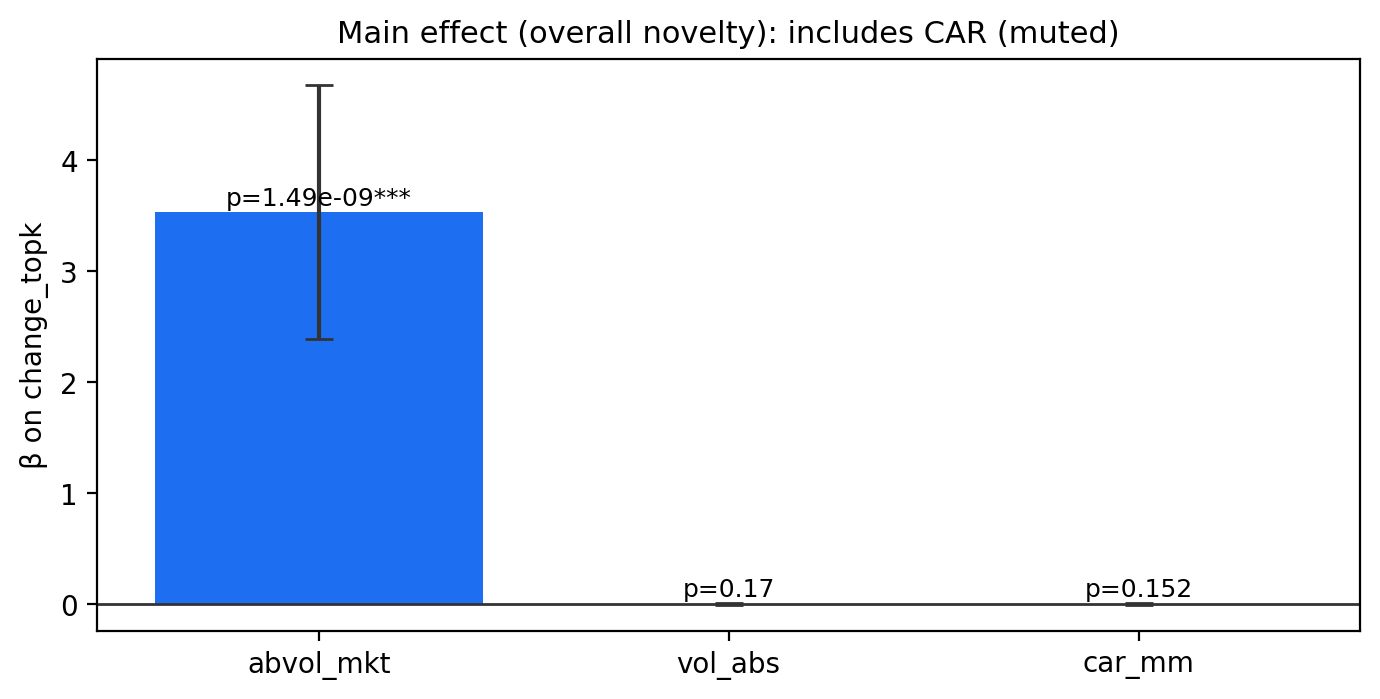
\includegraphics[width=0.92\textwidth]{figures/slide7_main_effect_ci_with_car.png}
  \caption{新規性（\texttt{change\_topk}）とイベント窓アウトカムの関係（係数と信頼区間）}
  \label{fig:main_effect_ci}
\end{figure}

\section{追加分析/頑健性確認}
本節では、（i）リスクカテゴリ別の異質性、（ii）プレトレンド、（iii）プラセボ（偽イベント日）等により、主結果の頑健性を検討する。

\subsection{カテゴリ別の異質性}
リスク文書をカテゴリ（地政学、災害/BCP、規制/コンプライアンス、人材、サイバー等）に分解し、
各カテゴリの新規性指標を用いて同様の回帰を行った。
異常出来高（\texttt{abvol\_mkt}）に対しては、災害/BCP（$\beta=2.078,\,p<0.001$）、
規制/コンプライアンス（$\beta=1.594,\,p<0.001$）、
人材（$\beta=0.807,\,p<0.01$）が正に有意であり、
新規性が注目を集める効果はカテゴリによって強弱があることが示唆される。

\begin{figure}[t]
  \centering
  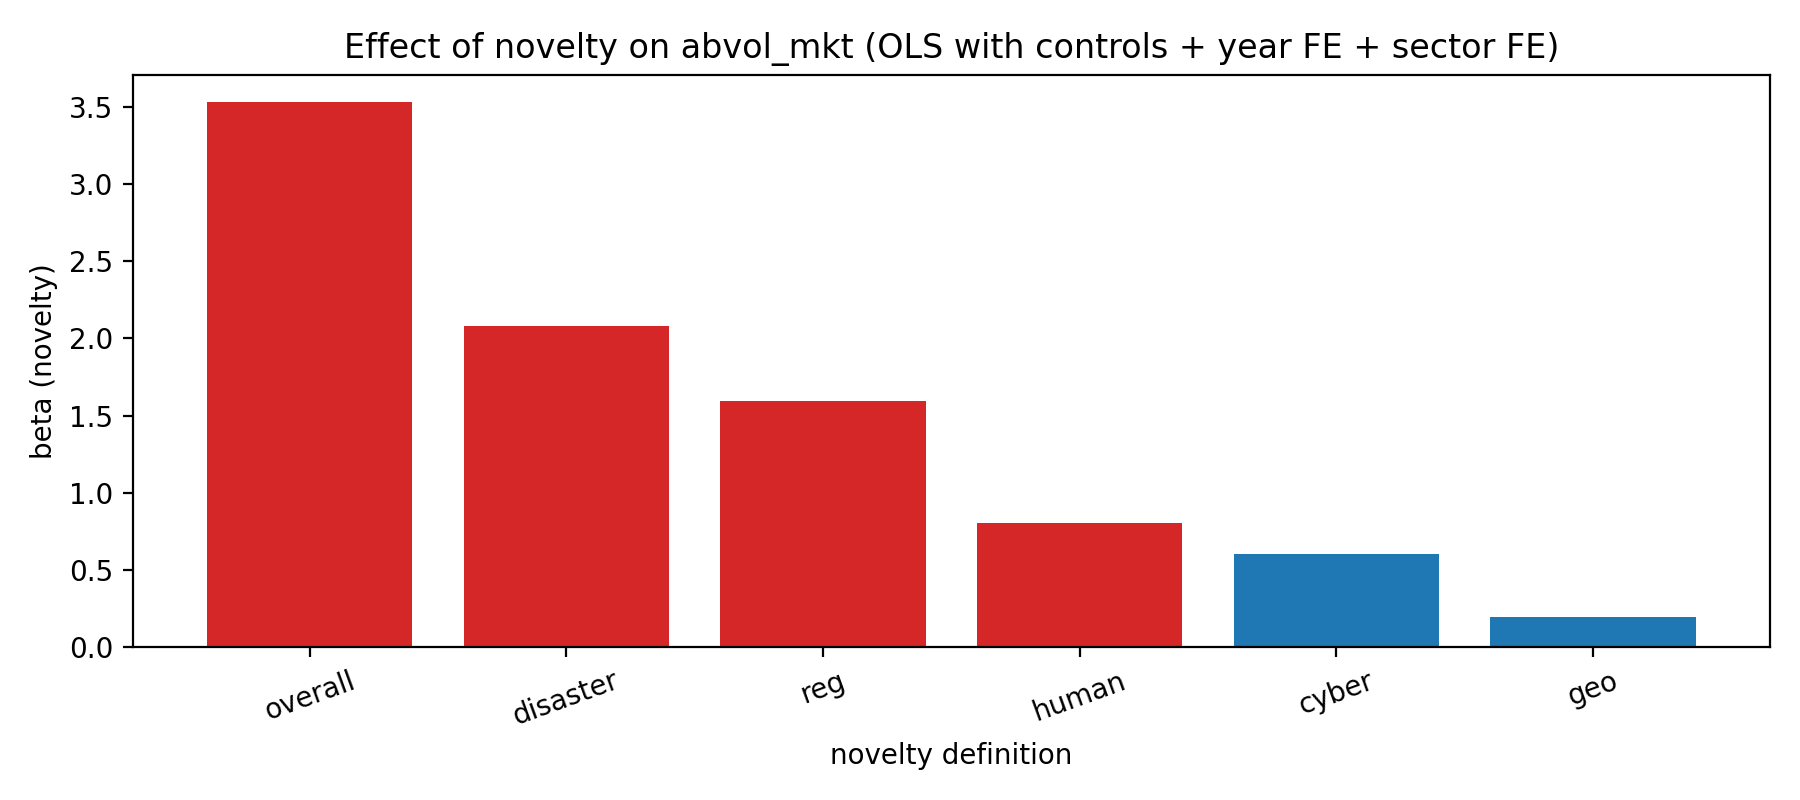
\includegraphics[width=0.92\textwidth]{figures/writeup_beta_abvol_by_category.png}
  \caption{カテゴリ別新規性と異常出来高（\texttt{abvol\_mkt}）の関係（係数と信頼区間）}
  \label{fig:abvol_by_category}
\end{figure}

\subsection{プレトレンド（事前窓）}
提出日の反応が、提出以前からのトレンド（事前窓）と区別できているかを確認するため、
事前窓（例：$-3,-1$）で算出したアウトカムと新規性の関係を推定した。
結果として、事前窓の異常出来高は新規性と強く相関し（$\beta=4.696,\,p<0.001$）、
提出日以前から注目が高い文書ほど新規性も高い可能性が示された。
この点は、新規性の解釈（情報の希少性だけでなく、企業・状況の背景要因を反映している可能性）において重要である。

\subsection{プラセボ（偽イベント日）と仕様変更}
さらに、イベント日を提出日からランダムにシフトした偽イベント日（プラセボ）を用い、
同一の推定仕様で「偽イベントでも同様の関係が出るか」を確認した。
仕様によってはプラセボ側の係数も一定の大きさを持つ場合があり、推定結果の解釈には注意が必要である。
また、企業固定効果を導入する仕様や、事前窓のアウトカムを統制変数として加える仕様では、
主結果（\texttt{abvol\_mkt} の正の関係）が弱まる傾向が確認された。

\subsection{外生ショック年ダミーを用いた追加分析}
外部イベント（ショック年）を用いた相互作用の推定も行い、
災害カテゴリ等における関係の変化を確認した。
図\ref{fig:shock_disaster}は、災害カテゴリに関する推定例を示す。

\begin{figure}[t]
  \centering
  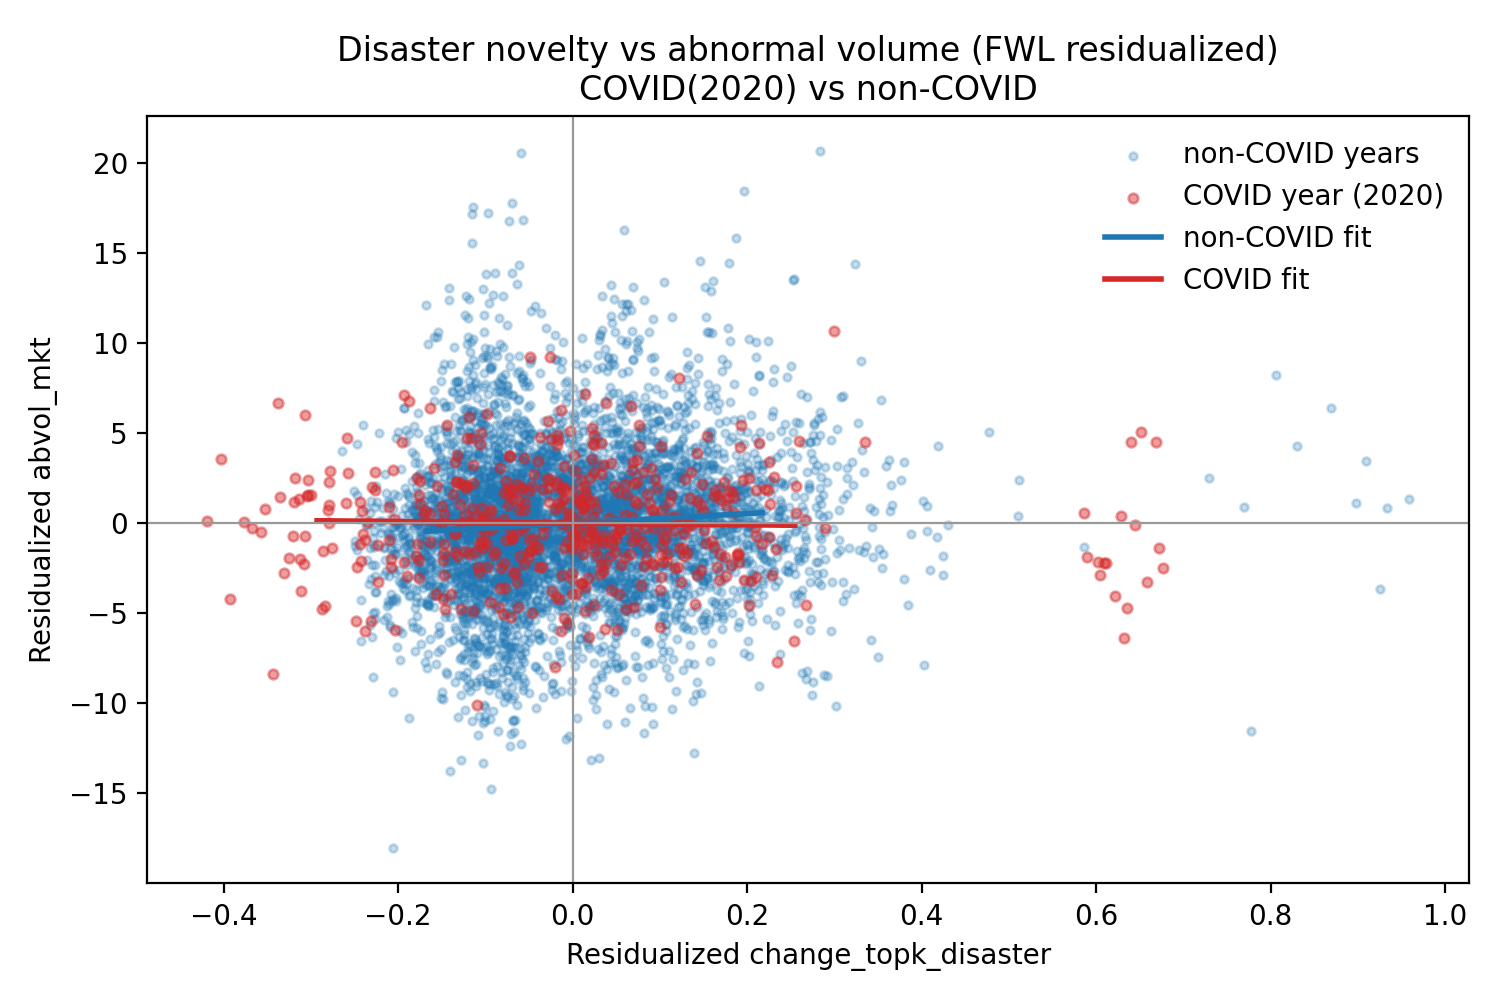
\includegraphics[width=0.92\textwidth]{figures/shock_disaster_scatter_fwl.png}\par
  \medskip
  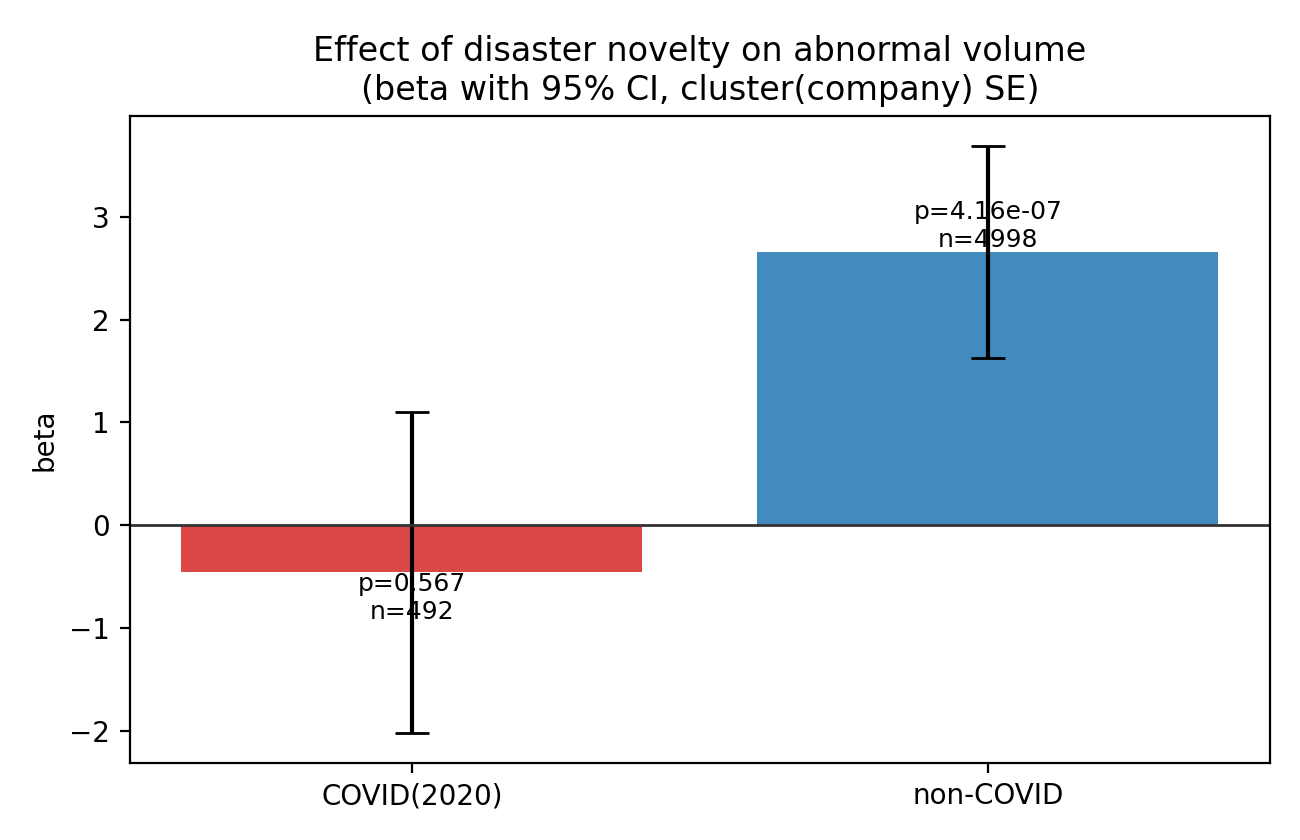
\includegraphics[width=0.92\textwidth]{figures/shock_disaster_beta_ci.png}
  \caption{外生ショック年を用いた推定例（災害カテゴリ）}
  \label{fig:shock_disaster}
\end{figure}



\chapter{考察}

\section{結果の解釈}
第3章の主結果は、リスク開示の新規性（\texttt{change\_topk}）が、価格反応（\texttt{car\_mm}）よりも投資家の注目（異常出来高：\texttt{abvol\_mkt}）と強く結びつくことを示した。これは、リスク情報の更新が直ちに株価水準を大きく変化させるというよりも、まず市場参加者の注意配分や情報探索行動を通じて現れる可能性を示唆する。すなわち、有価証券報告書の「事業等のリスク」欄の更新は、投資家にとって新情報の可能性がある一方、短期の価格調整としては限定的であり、注目の喚起として観測されやすいという解釈である。

一方で、不確実性指標（\texttt{vol\_abs}）および価格反応（\texttt{car\_mm}）が同一仕様で明確に有意でなかった点は、いくつかの説明が考えられる。第一に、リスク開示はネガティブ情報の告知であるだけでなく、リスクの所在を整理し、投資家の理解を促すという意味で情報環境の改善として評価され得る。したがって、価格反応の符号や大きさは一意ではなく、平均的には相殺されて小さく見える可能性がある。第二に、有価証券報告書の提出日前後には、同日または近接するIR開示や業績情報が同時に存在し得るため、提出日イベントにおける純粋な効果の抽出が難しい。第三に、価格への反映は即時ではなく遅行的である可能性もある。

\section{先行研究との比較}
先行研究では、リスク開示の量や語彙に基づく指標が、株式リスクや市場反応と関連し得ることが示されてきた\cite{Campbell2014}。また、リスク要因の更新（追加・削除）が不確実性と結びつく可能性も報告されている\cite{Lyle2023}。本研究は、従来の頻度や単純な差分では捉えにくい「意味的更新」に焦点を当て、埋め込みベースの類似度で新規性を定量化した点で、これらの研究の流れと整合的である。

ただし、本研究の結果は、価格反応（CAR）よりも注目度（出来高）で関係が強く観測された。これは、リスク情報の更新がまず注意の喚起として現れるという点で、情報処理・注意制約の議論と整合的である。他方、価格反応が弱いことは、リスク開示が既に市場に織り込まれている、あるいは提出日近傍の情報が多く識別が難しい、といった可能性も含む。したがって、先行研究の示す平均的な価格反応と単純に比較するのではなく、測定対象（リスク欄に限定した意味的更新）、市場（日本株）、イベント定義（提出日）といった制度的差異を踏まえた解釈が必要である。

\section{含意}
本研究の含意は、投資家行動と開示実務の両面にある。第一に、リスク欄の「新規性」は、少なくとも短期的には投資家の注目を喚起しやすい。したがって、投資家の情報処理過程を考える上で、開示の量だけでなく内容の更新度合いを捉えることが有用である。第二に、企業にとっては、形式的な記述の反復（いわゆるボイラープレート）よりも、状況変化に応じた具体的な更新が市場参加者の注意を引く可能性が示唆される。これは、規制対応としての開示に留まらず、投資家コミュニケーションとしての開示の質を高める方向性と整合的である。

一方で、注目の喚起が必ずしも価格の下落や不確実性の上昇につながらない可能性も示された。リスク開示の更新は、リスクの顕在化の兆候である場合もあれば、リスク管理や説明責任の強化（理解の促進）である場合もある。したがって、実務的には、更新内容の性質（リスクの増大を示すのか、管理の改善を示すのか）を区別して分析することが望ましい。

\section{限界と課題}
本研究にはいくつかの限界がある。第一に、推定された関係は、厳密な因果効果ではなく提出日周辺の統計的関連として解釈すべきである。新規性は企業の実態変化と同時に生じ得るため、交絡を完全に排除することは難しい。第3章で示したように、事前窓（プレトレンド）でも新規性とアウトカムが相関する場合があり、これは「新規性が高い文書は、提出以前から注目されやすい」といった背景要因の存在を示唆する。

第二に、提出日をイベント日とする設計は制度的に自然である一方、同日・近接日に他の情報（決算や適時開示等）が混在する可能性がある。第三に、新規性指標は埋め込みモデルと前処理（チャンク分割、トークン化等）に依存し、モデル選択や設定変更により値が変化し得る。第四に、カテゴリ別分析は、カテゴリ定義や分類精度、カテゴリ間の相関の影響を受ける。

以上を踏まえ、今後は（i）より強い外生性を持つショックや制度変更を利用した識別、（ii）提出日以外の情報公開タイミングも含めた設計、（iii）新規性の内容（新しいリスクの追加、既存リスクの強調、表現の具体化等）のタイプ分類、（iv）投資家属性やニュース環境を考慮した反応の異質性分析、などにより解釈と外的妥当性を高める必要がある。



\chapter{結言}

\section{結論}
本研究は、日本企業の有価証券報告書「事業等のリスク」欄に着目し、前年からの内容更新（新規性）を埋め込みベースの意味的類似度により定量化した上で、提出日周辺の市場反応との関係を検証した。主な結果は以下のとおりである。

第一に、リスク開示の新規性は、価格反応（CAR）よりも投資家の注目（異常出来高）と強く結びついた。すなわち、新規性の高いリスク開示ほど提出日周辺で取引が活発化する傾向が確認された。第二に、不確実性指標およびCARについては、同一の基本仕様では統計的に明確な関係が確認されず、リスク開示更新の効果が平均的な価格調整としては限定的である可能性が示唆された。第三に、カテゴリ別では、災害/BCP、規制/コンプライアンス、人材等で注目度との関係が比較的強く、リスク種類により反応が異なる可能性が示された。

\section{貢献の整理}
本研究の貢献は次の3点に整理できる。第一に、開示研究において「量」ではなく「更新（新規性）」に焦点を当て、日本の有価証券報告書リスク欄における年度間の意味的変化を扱った点である。第二に、チャンク分割と埋め込みベース類似度を用いて、言い換えや表現揺れを一定程度吸収しつつ新規性を測定する枠組みを提示した点である。第三に、市場反応を価格反応だけでなく注目度・不確実性の複数指標で検証し、リスク開示の新規性がどの側面に現れやすいかを識別した点である。

\section{今後の展望}
今後の課題として、第一に識別の強化が挙げられる。外生的ショックや制度変更、あるいは開示規制の改定等を利用し、新規性の変動がより外生的となる状況で検証することが望ましい。第二に、提出日以外の情報公開タイミングを含め、リスク情報が市場に取り込まれるプロセスをより精緻に捉える必要がある。第三に、新規性を一つのスコアに集約するだけでなく、追加・削除・具体化・強調といった更新タイプの分類により、どのタイプの更新が注目や不確実性に結びつくのかを検証することが重要である。第四に、投資家属性、ニュース環境、業種特性等による反応の異質性を体系的に分析し、外的妥当性を高めることが課題である。




% ---- Acknowledgements ----
\clearpage
\chapter*{謝辞}
\addcontentsline{toc}{chapter}{謝辞}
本研究の遂行にあたり、指導教員の野口怜先生には、研究テーマの設定から分析設計、結果の解釈、論文執筆に至るまで終始丁寧なご指導を賜りました。先生から頂いた数々のご助言は、本研究の方向性を定め、議論を深める上で大きな支えとなりました。ここに記して深く感謝申し上げます。

最後に、日頃より温かく見守り、学業と研究活動を支えてくれた家族に深く感謝いたします。

% ---- References ----
\clearpage
% thebibliography 環境（references.tex）側で見出しを出す（重複防止）
\renewcommand{\bibname}{参考文献}
\begin{thebibliography}{99}

% 目次に「参考文献」を載せる（見出しは thebibliography が自動生成）
\addcontentsline{toc}{chapter}{参考文献}

  \bibitem{Vaswani2017}
  A.~Vaswani, N.~Shazeer, N.~Parmar, J.~Uszkoreit, L.~Jones, A.~N.~Gomez, L.~Kaiser, and I.~Polosukhin,
  ``Attention Is All You Need,''
  \textit{arXiv preprint}, 2017.

  \bibitem{NelsonPritchard2007}
  K.~K.~Nelson and A.~C.~Pritchard,
  ``Litigation Risk and Voluntary Disclosure: The Use of Meaningful Cautionary Language,''
  \textit{SSRN Electronic Journal}, 2007.
  (DOI: \url{https://doi.org/10.2139/ssrn.998590})

  \bibitem{Campbell2014}
  J.~L.~Campbell, H.~Chen, D.~S.~Dhaliwal, H.~Lu, and L.~B.~Steele,
  ``The Information Content of Mandatory Risk Factor Disclosures in Corporate Filings,''
  \textit{Review of Accounting Studies}, 19(1), pp.~396--455, 2014.
  (DOI: \url{https://doi.org/10.1007/s11142-013-9258-3})

  \bibitem{HopeHuLu2016}
  O.-K.~Hope, D.~Hu, and H.~Lu,
  ``The Benefits of Specific Risk-Factor Disclosures,''
  \textit{Review of Accounting Studies}, 21(4), pp.~1005--1045, 2016.
  (DOI: \url{https://doi.org/10.1007/s11142-016-9371-1})

  \bibitem{Filzen2015}
  J.~J.~Filzen,
  ``The Information Content of Risk Factor Disclosures in Quarterly Reports,''
  \textit{Accounting Horizons}, 29(4), pp.~887--916, 2015.
  (DOI: \url{https://doi.org/10.2308/acch-51175})

  \bibitem{Lyle2023}
  M.~R.~Lyle, E.~J.~Riedl, and F.~Siano,
  ``Changes in Risk Factor Disclosures and the Variance Risk Premium,''
  \textit{The Accounting Review}, 98(6), pp.~327--352, 2023.
  (DOI: \url{https://doi.org/10.2308/TAR-2021-0174})

  \bibitem{Noda2016}
  野田 健太郎,
  「有価証券報告書における定性情報の分析と活用―リスクの多様化にともなう望ましい対話のあり方―」,
  \textit{経済経営研究}, Vol.37 No.1, 日本政策投資銀行設備投資研究所, 2016年5月.
  (\url{https://www.dbj.jp/ricf/pdf/research/DBJ_EconomicsToday_37_01.pdf})

  \bibitem{SatoIkedaInoue2021}
  佐藤 隆清・池田 直史・井上 光太郎,
  「有価証券報告書のテキストマイニングによる株式のリスクファクター分析」,
  \textit{証券アナリストジャーナル}, 2021年1月号, pp.~99--111.
  (\url{https://www.saa.or.jp/dc/sale/apps/journal/JournalShowDetail.do?goDownload=&itmNo=37464})

  \bibitem{KravetMuslu2013}
  T.~Kravet and V.~Muslu,
  ``Textual Risk Disclosures and Investors' Risk Perceptions,''
  \textit{Review of Accounting Studies}, 18(4), pp.~1088--1122, 2013.
  (DOI: \url{https://doi.org/10.1007/s11142-013-9228-9})

  \bibitem{LoughranMcDonald2016}
  T.~Loughran and B.~McDonald,
  ``Textual Analysis in Accounting and Finance: A Survey,''
  \textit{Journal of Accounting Research}, 54(4), pp.~1187--1230, 2016.
  (DOI: \url{https://doi.org/10.1111/1475-679X.12123})

  \bibitem{Dyer2017}
  T.~Dyer, M.~Lang, and L.~Stice-Lawrence,
  ``The Evolution of 10-K Textual Disclosure: Evidence from Latent Dirichlet Allocation,''
  \textit{Journal of Accounting and Economics}, 64(2--3), pp.~221--245, 2017.
  (DOI: \url{https://doi.org/10.1016/j.jacceco.2017.07.002})

  \bibitem{Devlin2019}
  J.~Devlin, M.-W.~Chang, K.~Lee, and K.~Toutanova,
  ``BERT: Pre-training of Deep Bidirectional Transformers for Language Understanding,''
  \textit{arXiv preprint}, 2019.
  (\url{https://arxiv.org/abs/1810.04805})

  \bibitem{ReimersGurevych2019}
  N.~Reimers and I.~Gurevych,
  ``Sentence-BERT: Sentence Embeddings using Siamese BERT-Networks,''
  \textit{arXiv preprint}, 2019.
  (\url{https://arxiv.org/abs/1908.10084})

  \bibitem{Wang2022E5}
  L.~Wang, N.~Yang, X.~Huang, L.~Yang, and F.~Wei,
  ``Text Embeddings by Weakly-Supervised Contrastive Pre-training,''
  \textit{arXiv preprint}, 2022.
  (\url{https://arxiv.org/abs/2212.03533})

\end{thebibliography}




% ---- Appendix (optional) ----
\clearpage
\appendix
\chapter{付録}

\section{分析で用いた主な変数の定義（概要）}
本研究で用いた主要変数の概要を、再現性の観点から補足する。

\subsection{リスク開示の新規性（Novelty）}
有価証券報告書「事業等のリスク」欄を一定長のテキスト・チャンクに分割し、当年チャンクと前年チャンク集合の間で埋め込み類似度を計算する。
各当年チャンクについて前年集合に対する最大類似度を求め、\(1-\max(\mathrm{sim})\) をチャンク単位の新規性として定義する。
企業年の新規性指標は、上位 \(k\%\) のチャンク新規性の平均（\texttt{change\_topk}）として集約する。

\subsection{市場反応（アウトカム）}
提出日をイベント日とし、イベント窓（例：\(-1,+1\)）で以下のアウトカムを算出する。

\begin{itemize}
  \item \texttt{abvol\_mkt}：市場調整後の異常出来高（投資家の注目度の代理変数）
  \item \texttt{vol\_abs}：異常収益の絶対値集計（不確実性の代理変数）
  \item \texttt{car\_mm}：市場モデルに基づく累積異常収益（価格反応）
\end{itemize}

\section{再現可能性のための補足（実行手順の最小要約）}
分析はPythonを中心に実施し、データ取得から前処理、指標構築、推定、図表生成までをノートブックで管理した。
また、重い処理（埋め込み計算や疑似イベントの反復推定等）については中間成果物のキャッシュを活用し、乱数シードを固定して再現性を担保した。
実行環境・手順の詳細は、リポジトリ内の \texttt{README} およびノートブックに記載の手順に従う。

\section{追加の頑健性確認（本文の補足）}
本文で示した主結果に加え、以下の観点で追加検証を行った。

\begin{itemize}
  \item 事前トレンド（pre-trend）の確認
  \item 偽イベント日（placebo）による比較
  \item 固定効果（年、業種、企業）の導入有無による結果の安定性
\end{itemize}

これらの追加分析の数値結果や図表は、リポジトリの出力（例：\texttt{outputs/} 配下）として保存しており、主要な含意は本文でも要約した。




\end{document}


